\chapter{Introducción}
 


\section{Un poco de historia}

Plagiar consiste en hacer uso del trabajo o las ideas de otra persona como si fuesen propias \cite{plagio_rae}.
\newline
La palabra plagio proviene del latín "plagiarus" que significa secuestrador y "plaga": "trampa, red" \cite{plagio_etim}. 
\newline
Esta infración empezó a cobrar importancia cuando las palabras e ideas empezaron a ser vistas como propiedad a través de publicaciones . Esto ocurrió a comienzos del siglo dieciocho conforme el arte y la literatura empezaron a verse como expresión de individualidad y personalidad de su autor \cite{plagio_paper}.
\newline
Por esta razón en 1709 se creó la primera ley inglesa de copyright (el Estatuto de la Reina Ana) que con el tiempo fueron incorporando más y más paises en su legislación, siendo Estados Unidos en 1891 el último gran país en incorporar una ley para proteger a sus autores \cite{plagio_historia}.
\newline
En el ámbito académico se procede de distintas formas para penalizar el plagio entre los estudiantes dependiendo de la institución.
\newline
En universidades estadounidenses por ejemplo, las penalizaciones pueden variar dependiendo de si la copia ha sido accidental (reducción de la calificación del estudiante) o intencional. En el caso de ser intencional normalmente se procederá suspendiendo la entrega o la asignatura e incluso expulsando al alumno de la universidad. 
\newline

En el caso de la Universidad de Granada según el Artículo 15 ''Originalidad de los trabajos y pruebas.'' de la normativa de evaluación y de calificación de los estudiantes de la Universidad de Granada, en caso de detectarse plagio esto ''conllevará automáticamente la calificación numérica de cero en la asignatura en la que se hubiera detectado, independientemente del resto de las calificaciones que el estudiante hubiera obtenido'' \cite{normativa_plagio}.
\newline
En la actualidad el plagio también es un problema que ocurre en archivos en código fuente, aunque su detección es más complicada ya que, por ejemplo, la copia se puede producir a nivel de estructura del programa. Además de esto, existen una gran cantidad de lenguajes de programación diferentes con sus características propias y con distintos niveles de abstracción, lo que dificulta aún más su detección ya que naturalmente es necesario que se tengan en cuenta las propias características del lenguaje (sus palabras reservadas, su control de flujo, cómo controlan la creación de objetos,...) a la hora de saber si dos programas escritos en el mismo lenguaje son o no similares.
\newline
Para resolver este problema existen diversas herramientas que automatizan la detección de plagio en código fuente basándose en los "tokens" del lenguaje, el número de veces que se llama a una función, la distancia entre dos secuencias de strings, etc.
\newline
Entre estas herramientas cabe destacar MOSS \cite{Moss_web}, JPLAG \cite{web_jplag}, SIM \cite{sim} y Plaggie \cite{plaggie}.

 
\section{Motivación}

R es un lenguaje de programación de alto nivel y un entorno de software interactivo pensado para computación estadística y gráficas\cite{whatisR}. R está basado en S y en Scheme por lo que también es bastante similar a Matlab.
\newline
R es gratis y de código abierto, no tiene restricciones de licencia, es compatible con Linux, Windows y Macintosh y tiene más de 4800 paquetes con funciones fáciles de usar.
\newline
Por estas razones R es un lenguaje que cada vez más gente usa y se enseña en más y más universidades.
\newline
Aunque su uso se esté expandiendo, todavía no existe una forma para detectar plagio en este lenguaje de forma eficaz y eficiente, ya que ninguna de las herramientas para detección de plagio existentes son compatibles con R tal y como podemos apreciar en la tabla comparativa en la Figura \ref{fig:figura1}. 

\bigskip

\begin{figure}[H] %con el [H] le obligamos a situar aquí la figura
\centering
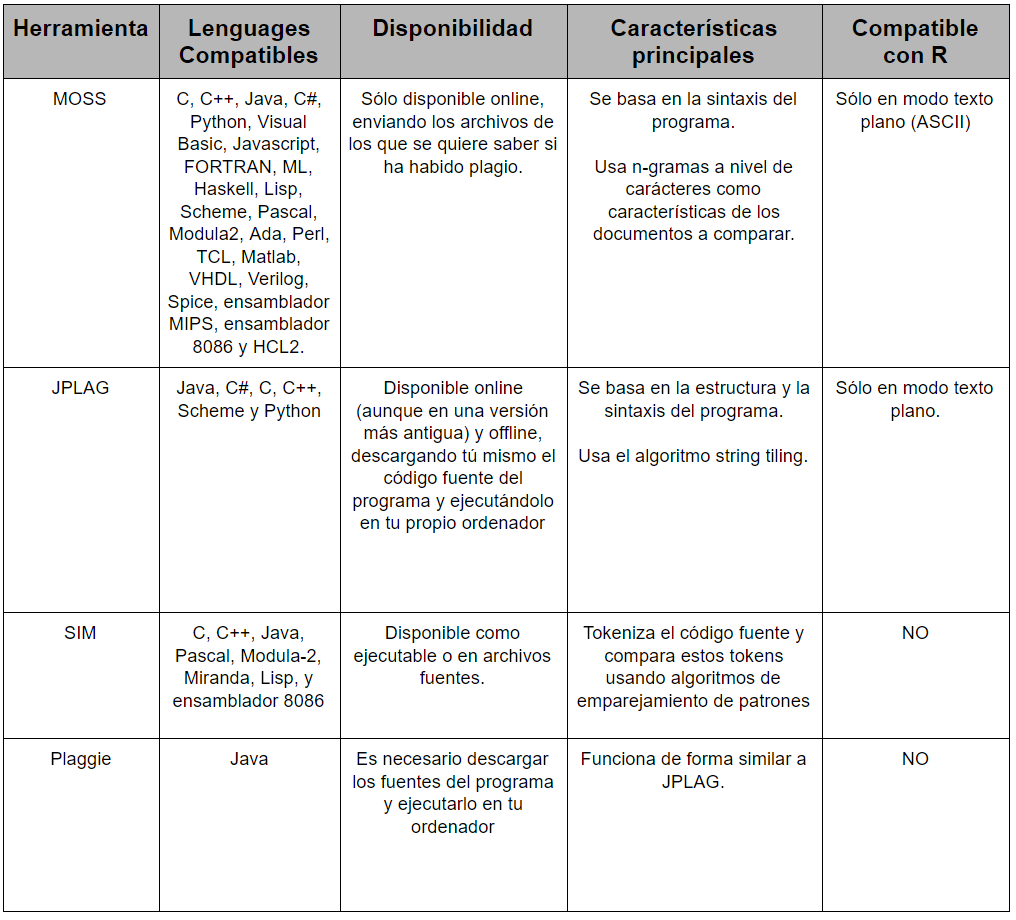
\includegraphics[scale=0.6]{imagenes/tabla_comparativa.png}  %el parámetro scale permite agrandar o achicar la imagen. En el nombre de archivo puede especificar directorios
\caption{Tabla comparativa de las herramientas para detección de plagio en código fuente más prominentes} \label{fig:figura1}
\end{figure}

\bigskip

Dado que, como podemos observar, no existe ninguna herramienta directa para R, hasta el momento lo que se ha hecho es detectarlo de forma manual o usando los detectores de plagio en modo texto plano.
\newline
La detección de forma manual requiere examinar uno a uno los archivos que mandan los alumnos comparándolos entre sí buscando similaridades en el código. Esto es demasiado lento y no efectivo en caso de que haya una gran cantidad de trabajos de alumnos ya que son demasiadas posibles comparaciones como para que el evaluador pueda tener en cuenta lo que han hecho todos los demás.
\newline
Por otra parte usar los detectores de plagio en modo texto plano, aunque sea rápido, pierde en eficacia ya que no tiene en cuenta las características propias del lenguaje y solo detectará plagio en caso de haberse hecho una copia literal.
\newline


\section{Objetivos}

El objetivo por tanto de este trabajo es solucionar este problema adaptando una de las herramientas para detección de plagio disponibles a R.
\newline
Hemos elegido JPLAG como herramienta a adaptar dado que es por norma general la herramienta que da mejores resultados para la detección de plagio en lenguajes en los que sí es compatible y además es la más fácilmente modificable debido a que se estructura en distintos frontends de lenguajes independientes del algoritmo principal de comparación y a que podemos descargar y modificar su código fuente.
\newline
Podemos dividir este objetivo en los siguiente sub-objetivos:
\begin{itemize}
	\item Estudiar y entender el funcionamiento de la estructura de clases de JPLAG
	\item Añadir un frontend para que JPLAG pueda procesar archivos en R.
	\item Modificar dicho frontend para que JPLAG reciba correctamente los "tokens" propios del lenguaje.
	\item Realizar las pruebas necesarias para verificar que se ha adaptado JPLAG correctamente a R y obtiene mejores resultados que en texto plano.
\end{itemize}
	




\section{Estructura del documento}

Este proyecto de fin de grado está estructurado en ocho capítulos que explican todo el trabajo que se ha llevado a cabo para la adaptación de JPLAG a R:
\begin{enumerate}
\item \textbf{Introducción}: en este capítulo se explica el problema en cuestión que queremos resolver.
\item \textbf{Planificación}: organización de mi tiempo y mis recursos para la realización de este trabajo y presupuesto.
\item \textbf{Análisis}: especificación de los requisitos funcionales y no funcionales, y los casos de uso de la tarea en cuestión. 
\item \textbf{Elección de herramientas}: en este capítulo se muestran las herramientas disponibles para la detección de plagio, se explica por qué se han elegido JPLAG y MOSS y se detalla cómo funcionan éstas.
\item \textbf{Implementación}: aquí se explican las partes más importantes del desarrollo, es decir, qué ha sido necesario añadir y modificar para la creación de nuestro frontend y para que éste procese archivos en R.
\item \textbf{Ejecución y Pruebas}: instrucciones sobre cómo ejecutar JPLAG y MOSS, pruebas que se han llevado a cabo con nuestra versión nueva de JPLAG, comparándola con la versión antigua y con MOSS, y análisis de estas pruebas.
\item \textbf{Conclusiones y trabajo futuro}: conclusiones de lo hecho en el trabajo y posibles mejoras que se puedan hacer al frontend.
\item \textbf{Apéndice}: código fuente añadido a JPLAG.
\end{enumerate}
